\documentclass[handout,table]{beamer}

% replace "handout" with "notes" to get pauses back
% Import packages:
\usepackage{graphicx}
%\graphicspath{{../Figures/}}
\usepackage{xcolor}
\usepackage{colortbl}
\usepackage{url}
\usepackage[english]{babel}
\usepackage[latin1]{inputenc}
\usepackage{times}
\usepackage[T1]{fontenc}
\usepackage{subfigure}% subcaptions for subfigures
\usepackage{subfigmat}% matrices of similar subfigures
\usepackage{multirow}


% Set theme templates:
\mode<presentation> {
 \usetheme{default}
 \usecolortheme{default}
 \useoutertheme{default}
 \useinnertheme{default}
 \setbeamercovered{invisible} 
 \setbeamertemplate{frametitle}[default][none]
 \setbeamertemplate{items}[circle]
 \setbeamertemplate{blocks}[rounded][shadow=true]
}
    
% Define some Stanford University Colors:
\xdefinecolor{cardinal}{RGB}{164, 0, 29}
\xdefinecolor{sandstone}{RGB}{231,209,154}

% Set colors of slide components:
\usecolortheme[named=cardinal]{structure}
\setbeamercolor{frametitle}{fg=sandstone,bg=cardinal }
\setbeamercolor{title}{fg=cardinal}


% Background gradient:
%\beamertemplateshadingbackground{white!50}{cardinal!100}

% Remove navigation bar:
\beamertemplatenavigationsymbolsempty



% Set up the title page:
\title{\huge{\bf SU$^2$ Pre-Release Workshop}}
\author{ 
 { \bf Presented by Thomas D. Economon \\
\bf \footnotesize {Hosted by the SU$^2$ Development Team} \\ 
 {\tiny\itshape
 Aerospace Design Lab, Stanford University, Stanford, CA 94305, U.S.A.}}\\ 
% \and \\
% \ Mazyar Zeinali %\thanks{Researcher.}
% \ and Daniel Rutherford \\%\thanks{Senior Researcher.}\\
% {\tiny\itshape
% International Council on Clean Transportation, San Francisco, CA 94104, U.S.A.}
}
\date{ \huge January 17, 2012}
\logo{
\includegraphics[width=2.0in]{logo.pdf} }


% Start
\begin{document}

% Titlepage:
{ \usebackgroundtemplate{
\includegraphics[width=\paperwidth]{SU2_logo.pdf}}
  \logo{ }
  \begin{frame}
   \titlepage
  \end{frame} }

% Outline:
%\begin{frame}[t]
%  \frametitle{Outline \hfill  \small{ \insertframenumber/\inserttotalframenumber} }
%  \small{
%  \tableofcontents
%  }
%\end{frame}


%\section{Introduction}

\begin{frame}[t]
\frametitle{What is the SU$^2$ suite? \hfill  \small{ \insertframenumber/\inserttotalframenumber} }

\begin{columns} 
  \begin{column}{.7\textwidth}
\begin{itemize}
\item \textcolor{cardinal}{\underline S}tanford \textcolor{cardinal}{\underline U}niversity \textcolor{cardinal}{\underline U}nstructured

\pause

\item \textcolor{cardinal}{Open source suite for the analysis and control of arbitrary PDEs} using unstructured grids
\begin{itemize}
\item Computational Fluid Dynamics (CFD)
\item Optimal Shape Design (OSD)
\item Mesh tools: adaptation, smoothing, deformation
\end{itemize}
\end{itemize}
  \end{column}
  \begin{column}{.3\textwidth}
\begin{figure}
\begin{center}
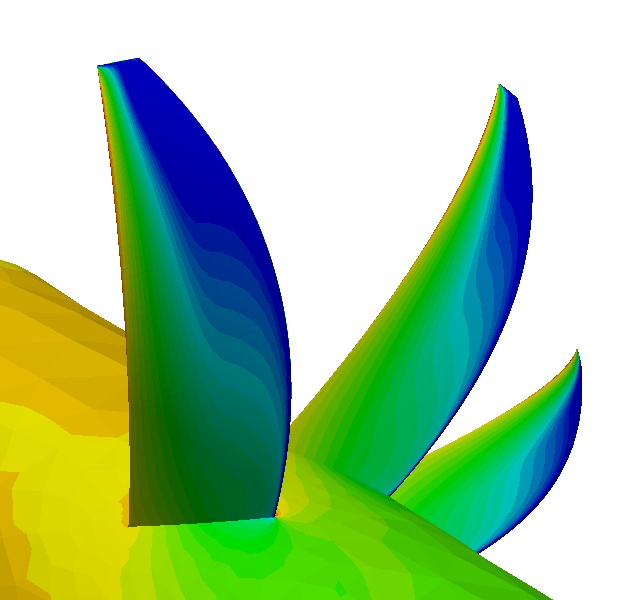
\includegraphics[width=1.0\textwidth]{rotor_closeup.png}
\label{wedge_mesh}
\end{center}
\end{figure}
  \end{column}
\end{columns}

\pause

\begin{block}{}
Our medium-term goal: Develop a \textcolor{cardinal}{leading solver in the unstructured CFD community}
\end{block}

\pause

\begin{itemize}
\item Written in a \textcolor{cardinal}{friendly C++ style with an object-oriented structure}, and MPI parallelization
\item Python driver scripts for coupling multiple SU$^2$ tools
\end{itemize}

\end{frame}

\begin{frame}[t]
\frametitle{Some features of the SU$^2$ flow solver \hfill  \small{ \insertframenumber/\inserttotalframenumber} }

\begin{block}{}
\textcolor{cardinal}{Unstructured, vertex-based solver for multiphysics simulations}. SU$^2$ can handle an arbitrary number of equations.
\end{block}

\begin{itemize}
\item<2-> Direct, adjoint, and linearized solvers for multiple equation sets
\item<3-> Compressible and incompressible solvers
\item<4-> Space integration (3D, and "real" 2D): JST, Roe, AUMS, HLLC
\item<5-> Time integration: Euler explicit and implicit, dual time stepping, Runge-Kutta
\item<6-> Turbulence models: SA and SST (on going activity).
\item<7-> Convergence acceleration via agglomeration Multigrid
\item<8-> Fully parallelized with MPI
\end{itemize}

\end{frame}

\begin{frame}[t]
\frametitle{What can the SU$^2$ suite do? \hfill  \small{ \insertframenumber/\inserttotalframenumber} }

{\bf Analysis}: Euler, Laminar Navier-Stokes, RANS, Multi-Species N-S, Rotating Frame Euler, Potential, Linearized and Adjoint Equations, Two phase flows...

\begin{figure}
\begin{center}
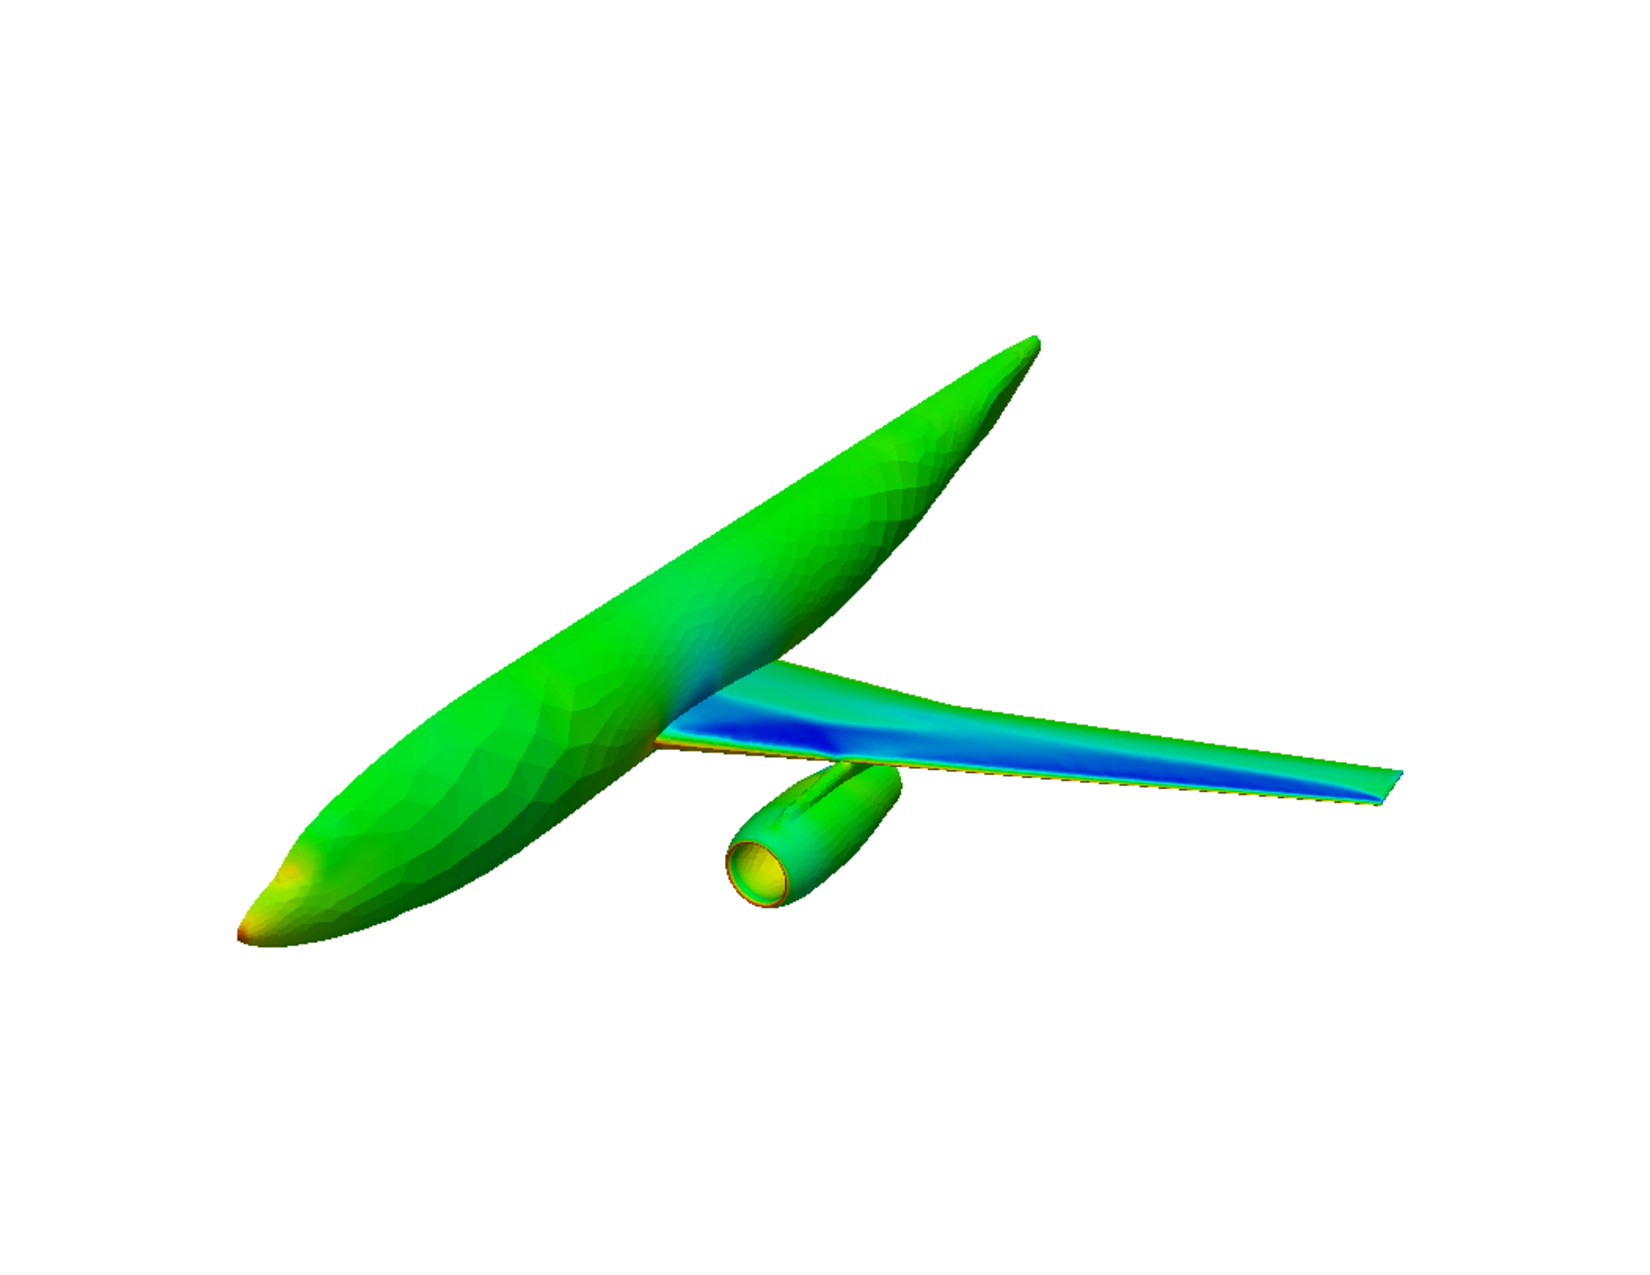
\includegraphics[width=3.0in]{DLRF6.pdf}
%\includegraphics[width=2.0in]{oneram6_pressure.png}
\label{analysis}
\end{center}
\end{figure}


\end{frame}


\begin{frame}[t]
\frametitle{What can the SU$^2$ suite do? \hfill  \small{ \insertframenumber/\inserttotalframenumber} }

{\bf Design}: Continuous Adjoint, Gradient Projection, Design Variable Definition, Mesh Deformation, Free Form Deformation, Shape Optimization (complete design loop)...

\begin{figure}
\begin{center}
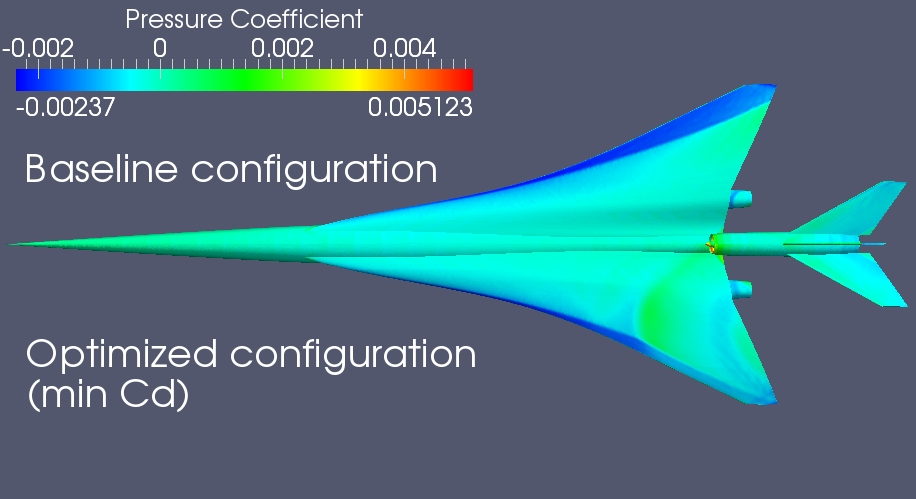
\includegraphics[width=3.5in]{Upper_CdDesign.jpg}
\label{design}
\end{center}
\end{figure}

\end{frame}



\begin{frame}[t]
\frametitle{ SU$^2$ Release Details \hfill  \small{ \insertframenumber/\inserttotalframenumber} }

Why an open-source license?

\begin{itemize}
\item To \textcolor{cardinal}{promote further research} by providing a proven platform
\item To \textcolor{cardinal}{improve and grow the code} based on the experience of users and the additions from developers
\end{itemize}

\pause

Why use SU$^2$?

\begin{itemize}
\item \textcolor{cardinal}{Available to {\it \bf ANYONE} for {\it \bf FREE }}
\item \textcolor{cardinal}{Code maintenance and support} provided by our lab and the open-source community
\item \textcolor{cardinal}{Developer-friendly C++ structure}, it is very simple to modify and build upon, including adding new equations
\end{itemize}

\end{frame}

\begin{frame}[t]
\frametitle{Workshop Agenda \hfill  \small{ \insertframenumber/\inserttotalframenumber} }

{\center

{\bf Introduction to SU$^2$}

\vspace{0.3in}

{\bf Hands-on Session: }

\vspace{0.05in}

{ Download \& Build on Your Machine}

\vspace{0.05in}

Run the Quick Start Tutorial

\vspace{0.05in}

Work Through Remaining Tutorials

\vspace{0.05in}

Attempt the Workshop Challenge

\vspace{0.3in}

{\bf Submit Feedback Before Leaving }

}


\end{frame}


\begin{frame}[t]
\frametitle{Workshop Goals \hfill  \small{ \insertframenumber/\inserttotalframenumber} }

\vspace{0.3in}
Our goals for the workshop are the following:

\begin{enumerate}
\item Introduce SU$^2$ and begin growing the user base 
\item Test the readiness of the code prior to release
\item Evaluate the effectiveness of the documentation
\end{enumerate}

\vspace{0.3in}

 Your feedback is vital to the success of this workshop! Please rate your experiences and add your comments in the embedded surveys. The SU$^2$ team will be available around the room during the hands-on session to help with the code and hear about your experience.

\end{frame}


\begin{frame}[t]
\frametitle{Workshop Challenge: 2-D Supersonic Wedge \hfill  \small{ \insertframenumber/\inserttotalframenumber} }

\vspace{-0.2in}

\begin{figure}
\begin{center}
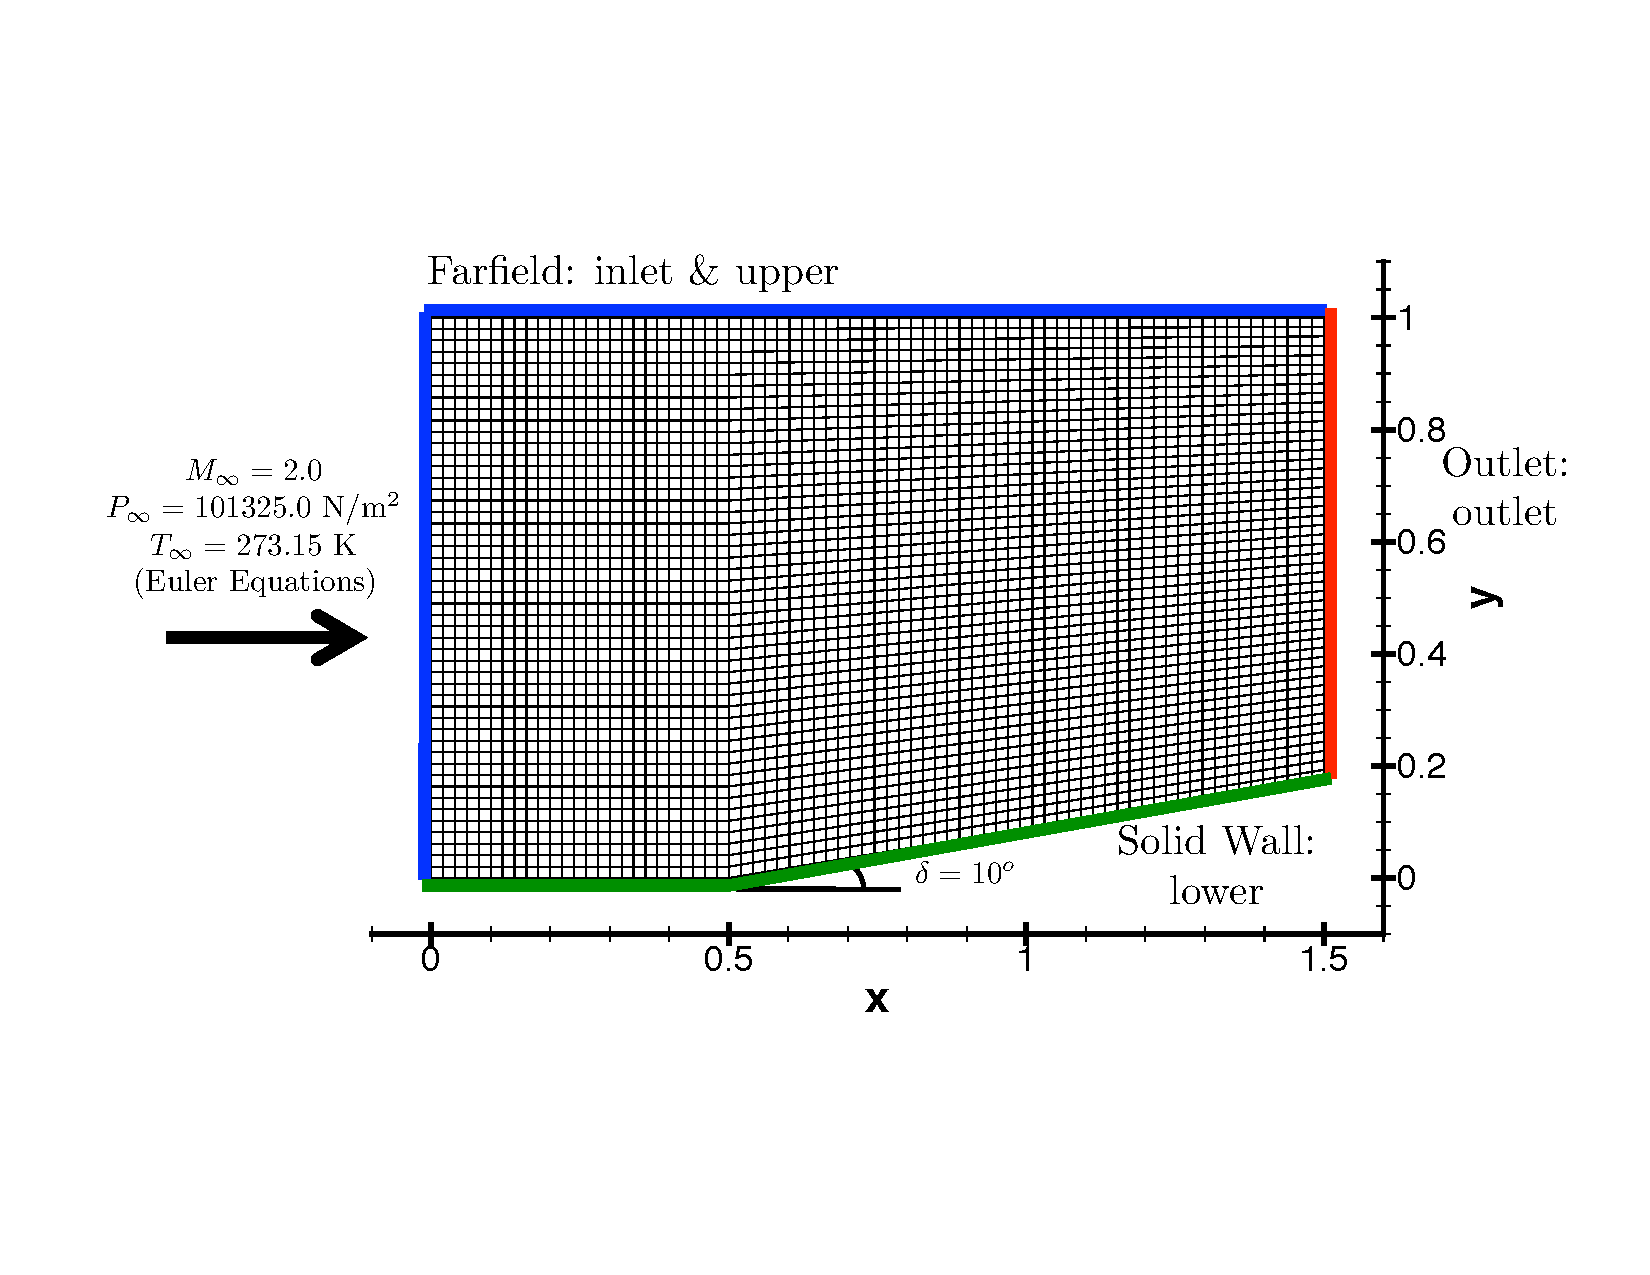
\includegraphics[width=4.0in]{mesh&bcs.pdf}
\label{wedge_mesh}
\end{center}
\end{figure}

\vspace{-0.25in}
\center
{\tiny After performing the tutorials, try to get this simple problem working on your own.

Download the mesh from within the documentation and start with the template configuration file. }

\end{frame}

\begin{frame}[t]
\frametitle{Workshop Challenge: 2-D Supersonic Wedge \hfill  \small{ \insertframenumber/\inserttotalframenumber} }


\begin{figure}
\begin{center}
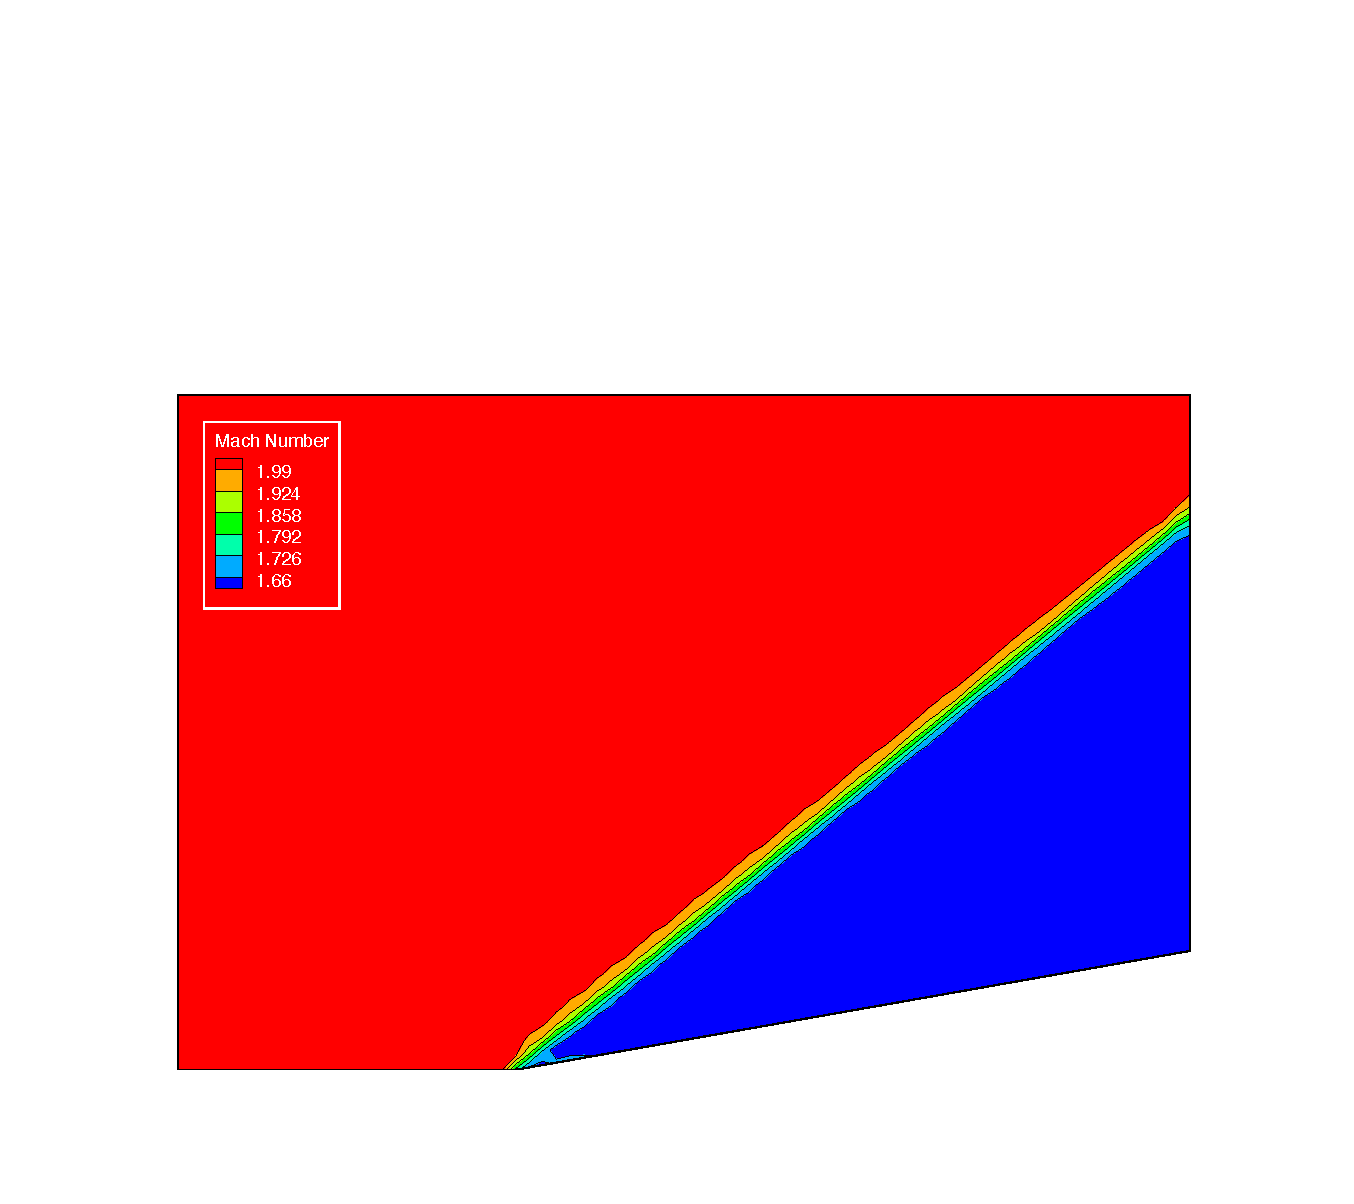
\includegraphics[width=3.5in]{wedge_mach.pdf}
\label{wedge_mach}
\end{center}
\end{figure}

\begin{columns}
\column{0.6\textwidth}
 Can you converge 5 orders of magnitude in fewer than 75 iterations?
\column{0.4\textwidth}
\end{columns}

\end{frame}



{ \usebackgroundtemplate{
\includegraphics[width=\paperwidth]{SU2_logo.pdf}}
  \logo{ }
  \begin{frame}

\begin{center}
   
  {\huge SU$^2$ Release: January 19, 2012 }
  
  \vspace{0.3in}
  
   The code, all of the documentation, and instructions for joining the user's mailing list can be found on the SU$^2$ home page:

  \vspace{0.3in}
  
{ \huge su2.stanford.edu }

   \vspace{0.3in}
   
Users are encouraged to join the SU$^2$ user's email list. This list will be used to communicate important information to users such as new releases and bug fixes.

   \vspace{0.3in}

   Contact the SU$^2$ Team at {\it susquared-dev@lists.stanford.edu}. \\ We appreciate any feedback!  
   
   \end{center}
  \end{frame} 
  }
  

\end{document}